%% LyX 2.2.4 created this file.  For more info, see http://www.lyx.org/.
%% Do not edit unless you really know what you are doing.
\documentclass[english]{article}
\usepackage{lmodern}
\usepackage[T1]{fontenc}
\usepackage[latin9]{inputenc}
\usepackage{geometry}
\geometry{verbose,tmargin=3cm,bmargin=3cm,lmargin=2.5cm,rmargin=2.5cm}
\usepackage{textcomp}
\usepackage{amstext}
\usepackage{graphicx}

\makeatletter

%%%%%%%%%%%%%%%%%%%%%%%%%%%%%% LyX specific LaTeX commands.
%% Because html converters don't know tabularnewline
\providecommand{\tabularnewline}{\\}

\makeatother

\usepackage{babel}
\begin{document}

\title{3F8: Inference\\
 Short Lab Report}

\author{Danut-Gabriel Buica}
\maketitle
\begin{abstract}

Given a set of classified data we want to be able to predict 
the class membership  of future data. Therefore, we built two types of classifier. We started with a linear clasifier and as expected we discovered that it does not optimally fit our data, although it will serve as lower bound in terms of performance. We continued with a non-linear, more complex classifier that expands the features of our data. By experimated with different parameters, we determined that at the cost of computational power and more tuning, we can achive far better prediction rates. 

\end{abstract}

\section{Introduction}
\begin{enumerate}
\item Given a set of classified data, we want to predict the class of futere data point. During this lab we will implement a clasifier that will split our data into 2 clases. We will aplly it to a simple data set to assess its performance.
\item First we will start with a simple linear classifier and see how well it performs on our data. Then, we will try a more complicated non-linear model that expands the features of our data points. After recording the results for both cases, we will compare them and decide upon advatages and disadvatages of each model.
\end{enumerate}

\section{Exercise a)\label{sec:Exercise-a}}

In this exercise we have to consider the logistic classication model
(aka logistic regression) and derive the gradients of the log-likelihood
given a vector of binary labels $\mathbf{y}$ and a matrix of input
features $\mathbf{X}$. The gradient of the log-likelihood can be
writen as
\[
\frac{\partial\mathcal{L}(\beta)}{\partial\beta}=\sum_{n=1}^{N}\tilde{x}^{(n)}(y^{(n)} - \sigma(\beta^T\tilde{x}^{(n)}))\,
\]
\[
\frac{\partial\mathcal{L}(\beta)}{\partial\beta}=\mathbf{X}^T[\mathbf{y} - \sigma(\beta^T\mathbf{X})]]\,.
\]

\section{Exercise b)}

In this exercise we are asked to write pseudocode to estimate the
parameters $\beta$ using gradient ascent of the log-likelihood. Our
code should be vectorised. The pseudocode to estimate the parameters
$\beta$ is shown below:
\newpage
\begin{verbatim}
Function estimate_parameters:

   Input:  feature matrix X, labels y
   Output: vector of coefficients b
	
   Code:
    initialise b
    for i in range (steps) do
        gradient <- Transpose(X).(y - logistic(Transpose(b) . X)) 
        b <- b + learning_rate*gradient
    return b
\end{verbatim}
The learning rate parameter $\eta$ is chosen commonly by trial and error. A high learning rate can overshoot the maximum and oscullate around it. A small learning rate can lead to a slow converging rate and makes the algorithm computational unefficient. We can choose the learning rate by plotting the log-likelihood for increasing values of $ \eta $ and choose the first value for which the system does not oscillate. Another method of choosing the learning rate is to use a fuction which deacreses with the number of steps.

\section{Exercise c)}

In this exercise we visualise the dataset in the two-dimensional input
space displaying each datapoint's class label. The dataset is visualised
in Figure \ref{fig:data_visualisation}. By analising Figure \ref{fig:data_visualisation}
we conclude that a linear classifier cannot separate the two classes. Not being design for this type of data, this claifier would perform fairly poorly and it is garanted that we will experience missclassification of the data.

\begin{figure}[!h]
\begin{centering}
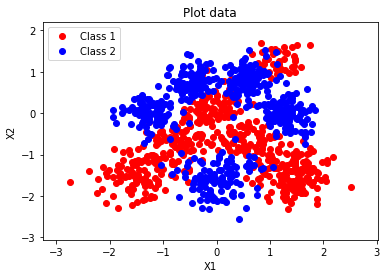
\includegraphics[width=0.3\paperwidth]{fig1}
\par\end{centering}
\caption{Visualisation of the data.\label{fig:data_visualisation} }
\end{figure}


\section{Exercise d)}

In this exercise we split the data randomly into training and test
sets with 800 and 200 data points, respectively. The pseudocode from
exercise a) is transformed into python code as follows:
\begin{verbatim}
w = np.random.randn(X_tilde_train.shape[ 1 ])
for i in range(n_steps):
    sigmoid_value = predict(X_tilde_train, w)
    Gradient = np.dot(np.transpose(X_tilde_train), (y_train - sigmoid_value))
    w += alpha * Gradient
return w
\end{verbatim}
We then train the classifier using this code. We fixed the learning
rate parameter to be $\eta=0.001$ . The average log-likelihood on the
training and test sets as the optimisation proceeds are shown in Figure
\ref{fig:learning_curves}. By looking at these plots we conclude
that we havechosen a good learning rate given that the plots converge relatively quickly(around 20 steps) without oscillations. Also, the similarity between the both of the plots shows that our model can be generalized to unseen data.

Figure \ref{fig:learning_curves} displays the visualisation of the
contours of the class predictive probabilities on top of the data.
This figure shows that we predict with higher probability that class 1 is in the bottom part of the data, while class 2 has a high probability to be located in the upper part. As expected, our classifier could not see the class 1 cluster in the upper right part and the class 2 cluster from the bottom of the data. 


\begin{figure}[!h]
\begin{centering}
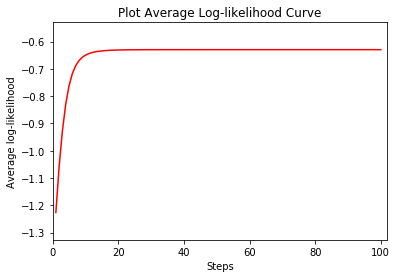
\includegraphics[width=0.3\paperwidth]{fig2}\hspace{1cm}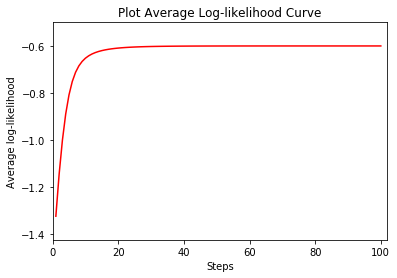
\includegraphics[width=0.3\paperwidth]{fig2b}
\par\end{centering}
\caption{Learning curves showing the average log-likelihood on the training
(left) and test (right) datasets.\label{fig:learning_curves} }
\end{figure}

\begin{figure}
\begin{centering}
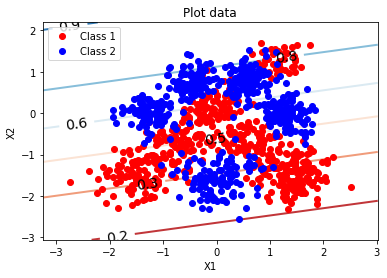
\includegraphics[width=0.3\paperwidth]{fig3}
\par\end{centering}
\caption{Visualisation of the contours of the class predictive probabilities.\label{fig:data_visualisation-1} }
\end{figure}


\section{Exercise e)}

The final average training and test log-likelihoods are shown in Table
\ref{tab:average_ll}. These results indicate that the model generalizes very well for unseen data (the final values are very close). The 2x2 confusion
matrices on the and test set is shown in Table \ref{tab:confusion_test}.
By analising this table, we conclude that the probabilities of correct predictions are much higher than the probabilities of missclassificasion. However, our contour plot shows that a linear boundary is not the optimal choice for classifying our data and that we need a non-linear classifier to achive higher probabilities of correct predictions.

\begin{table}[!h]
\centering{}%
\begin{minipage}[t]{0.49\columnwidth}%
\begin{center}
\begin{tabular}{c|c}
\textbf{Avg. Train ll} & \textbf{Avg. Test ll}\tabularnewline
\hline 
-0.628 & -0.609\tabularnewline
\hline 
\end{tabular} 
\par\end{center}
\caption{Average training and test log-likelihoods.\label{tab:average_ll}}
%
\end{minipage}%
\begin{minipage}[t]{0.49\columnwidth}%
\begin{center}
\begin{tabular}{cc|c|c}
 & \multicolumn{1}{c}{} & \multicolumn{1}{c}{$\hat{y}$} & \tabularnewline
 &  & 0 & 1\tabularnewline
\cline{2-4} 
$y$ & 0 & 0.71 & 0.29\tabularnewline
\cline{2-4} 
 & 1 & 0.25 & 0.75\tabularnewline
\cline{2-4} 
\end{tabular} 
\par\end{center}
\caption{Confusion matrix on the test set.\label{tab:confusion_test}}
%
\end{minipage}
\end{table}


\section{Exercise f)}

We now expand the inputs through a set of Gaussian radial basis functions
centred on the training datapoints. We consider widths $l=\{0.01,0.1,1\}$
for the basis functions. We fix the learning rate parameter to be
$\eta=\{0.01,0.001,0.0001\}$ for each $l=\{0.01,0.1,1\}$, respectively.
Figure \ref{fig:contours_l} displays the visualisation of the contours
of the resulting class predictive probabilities on top of the data
for each choice of $l=\{0.01,0.1,1\}$.
\begin{figure}[!h]
\begin{centering}
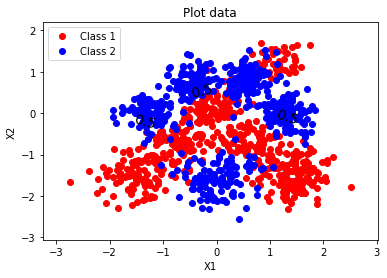
\includegraphics[width=0.32\textwidth]{l001}\hspace{0.15cm}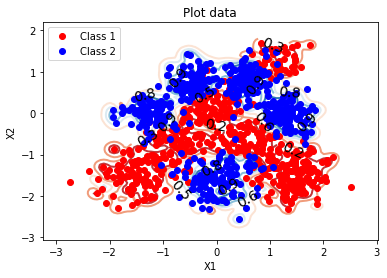
\includegraphics[width=0.32\textwidth]{l01}\hspace{0.15cm}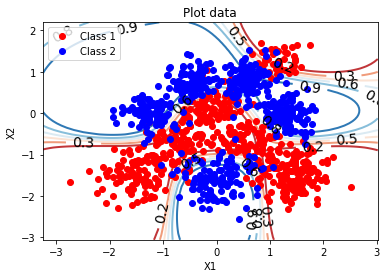
\includegraphics[width=0.32\textwidth]{l1}
\par\end{centering}
\caption{Visualisation of the contours of the class predictive probabilities
for $l=0.01$ (left), $l=0.1$ (middle), $l=1$ (right).\label{fig:contours_l} }
\end{figure}


\section{Exercise g)}

The final final training and test log-likelihoods per datapoint obtained
for each setting of $l=\{0.01,0.1,1\}$ are shown in tables \ref{tab:avg_ll_l_001},
\ref{tab:avg_ll_l_01} and \ref{tab:avg_ll_l_1}. These results indicate
that: the model with $ l = 0.01 $ fitted our data the best but it the least generalisable, having the worst log-likelihood on the test data. Also, it did not capture the structure of the data; the model with $ l=1 $ fitted our data the worst (the lowest log-likelihood for training data), but is the most generalisable having the best log-likelihood on unseen data; the model with $ l=0.1 $ has the classification bundaries very close to the clusters. Although, it would work well for data with low variance, it will fail for highly varied data. The 2 \texttimes{} 2 confusion matrices for the three models
trained with $l=\{0.01,0.1,1\}$ are show in tables \ref{tab:conf_l_001},
\ref{tab:conf_l_01} and \ref{tab:conf_l_1}. After analysing these
matrices, we can say that the first model performs very poorly, predicting only one class. Moreover, its accuracy is worse than that of the linear model. The second model, performs significantly better than the first one, but by setting the boundaries close to the clusters, the outside data tends to be classified all towards a single class. The last model is more robust and performs better than the previous ones. When we compare these results to those
obtained using the original inputs we conclude that our second and third non-linear models classify the data with higher accuracy. 

\begin{table}[!h]
\centering{}%
\begin{minipage}[t]{0.3\textwidth}%
\begin{center}
\begin{tabular}{c|c}
\textbf{Avg. Train ll} & \textbf{Avg. Test ll}\tabularnewline
\hline 
-0.010 & -0.665\tabularnewline
\hline 
\end{tabular}\caption{Results for $l=0.01$\label{tab:avg_ll_l_001}}
\par\end{center}%
\end{minipage}\hspace{0.5cm}%
\begin{minipage}[t]{0.3\textwidth}%
\begin{center}
\begin{tabular}{c|c}
\textbf{Avg. Train ll} & \textbf{Avg. Test ll}\tabularnewline
\hline 
-0.186 & -0.292\tabularnewline
\hline 
\end{tabular}\caption{Results for $l=0.1$\label{tab:avg_ll_l_01}}
\par\end{center}%
\end{minipage}\hspace{0.5cm}%
\begin{minipage}[t]{0.3\textwidth}%
\begin{center}
\begin{tabular}{c|c}
\textbf{Avg. Train ll} & \textbf{Avg. Test ll}\tabularnewline
\hline 
-0.201 & -0.223\tabularnewline
\hline 
\end{tabular}\caption{Results for $l=1$\label{tab:avg_ll_l_1}}
\par\end{center}%
\end{minipage}
\end{table}
\newpage
\begin{table}[!h]
\centering{}%
\begin{minipage}[t]{0.33\textwidth}%
\begin{center}
\begin{tabular}{cc|c|c}
 & \multicolumn{1}{c}{} & \multicolumn{1}{c}{$\hat{y}$} & \tabularnewline
 &  & 0 & 1\tabularnewline
\cline{2-4} 
$y$ & 0 & 0.97 & 0.03\tabularnewline
\cline{2-4} 
 & 1 & 0.85 & 0.15\tabularnewline
\cline{2-4} 
\end{tabular} 
\par\end{center}
\caption{Conf. matrix $l=0.01$.\label{tab:conf_l_001}}
%
\end{minipage}%
\begin{minipage}[t]{0.33\textwidth}%
\begin{center}
\begin{tabular}{cc|c|c}
 & \multicolumn{1}{c}{} & \multicolumn{1}{c}{$\hat{y}$} & \tabularnewline
 &  & 0 & 1\tabularnewline
\cline{2-4} 
$y$ & 0 & 0.93 & 0.07\tabularnewline
\cline{2-4} 
 & 1 & 0.13 & 0.86\tabularnewline
\cline{2-4} 
\end{tabular} 
\par\end{center}
\caption{Conf. matrix $l=0.1$.\label{tab:conf_l_01}}
%
\end{minipage}%
\begin{minipage}[t]{0.33\textwidth}%
\begin{center}
\begin{tabular}{cc|c|c}
 & \multicolumn{1}{c}{} & \multicolumn{1}{c}{$\hat{y}$} & \tabularnewline
 &  & 0 & 1\tabularnewline
\cline{2-4} 
$y$ & 0 & 0.94 & 0.06\tabularnewline
\cline{2-4} 
 & 1 & 0.08 & 0.92\tabularnewline
\cline{2-4} 
\end{tabular} 
\par\end{center}
\caption{Conf. matrix $l=1$.\label{tab:conf_l_1}}
%
\end{minipage}
\end{table}


\section{Conclusions}
\begin{enumerate}
\item Although 2 of the RBF models preformed better than the linear model, they are more computationally expensive. While the linear model converges quickly, our last RBF model took more than a few thousands of steps to converge, each step being more expansive due to the incresing size of the matrix. 
\item The RBF models require more tuning for RBF width, number of steps and learning rate. We have seen that a bad design can performe far worse than the linear model.
\item The linear model can gives us a better start of analysing the data set and can be considered a lower bound in terms of performance for more complicated models.
\end{enumerate}

\end{document}
